\chapter{Background} \label{backgorund}
The purpose of this chapter is to establish the background knowledge for this thesis. First, an introduction into the Domain Name System and the Hyptertext Transfer Protocol Secure including their vulnerabilities which are found up to date builds the basis of the chapter. Then, the functionality of the Transmission Control Protocol is introduced. The core of this chapter is the Section DNS over HTTPS, where the functionality, the strengths, and the vulnerabilities including a survey of the malware abusing the protocol are presented. In the end of the chapter, the platform SecGrid including a definition of PCAP-Files is shown.

\section{Domain Name System} \label{DNS}
The Domain Name System (DNS) is a protocol that is used to process naming resources in such a way that different users, networks etc. are all able to understand and identify the respective naming resource in their own language. An example for it is a user who types an URL into a web-browser. Since this URL is only understandable by human beings it has to be translated into a numerical IP-address and made understandable for the internet. This part is taken by the DNS which is a directory that administers the namespace of the whole internet. DNS has been introduced in 1993 and has since then become a crucial part of the internet \cite{RFC1035}. 

However, in this early time of the internet nearly no one thought about internet security and therefore lone DNS-queries are highly endangered to suffer cyber attacks. \cite{kim2020survey} found three different ways to view the vulnerabilities of DNS: the conceptual view, the structural view and the communication view. In the conceptual view, they applied a model for testing the information security called CIA Triad, which is structured into three parts: the confidentiality, the integrity and the availability. In all three parts this model showed that DNS is not secure and prone to attacks or failures of the servers due to the fact that DNS is not encrypted and has a hierarchical structure, such that anyone can tamper it. In the structural view, they found that the hierarchical tree structure of DNS servers makes it easier for attackers to attack several services used by a lot of users at the time. Another finding in this view was the exposure of DNS server information which is caused by insufficient security configurations of the DNS servers. This allows an attacker to send malicious data to the user and the user still beliefs that this data is secure. In the third view, the communication view they found that the packets are not secured through the usage of UDP, caching problems caused by Cache Poisoning can occur and there is a lack of protection against Distributed Denial of Service attacks. In summary, those three views show clearly that DNS is vulnerable in many aspects, which is the reason that in the evolution of the internet security there were many more security protocols developed.

\section{Hypertext Transfer Protocol Secure} \label{https}
The Hypertext Transfer Protocol (HTTP) \cite{RFC2616} was introduced in the early 1990s and has since then become a crucial part of the internet. It defines the communication of the web-server and the web-browser, communicates by using the Transmission Control Protocol (TCP) \cite{borman2014rfc7323} and works on the Application Layer of the OSI-Model \cite{silberschatz2013OSConcepts}. The Hypertext Transfer Protocol Secure (HTTPS) \cite{RFC2818} extends the HTTP, whereas the major difference between HTTPS and HTTP is that HTTPS additionally is encrypted by using Secure Sockets Layer (SSL) \cite{RFC6101} or its successor Transport Layer Security (TLS) \cite{RFC2246} protocol. HTTPS uses port 443 by default and its URLs start with "\textit{https://}". The common start of a TLS connection \cite{naylor2014costs} is a \textit{handshake} between server and client, where the Public Key Infrastructure (PKI) is used to first authenticate the server, afterwards a symmetric key for the session is generated by asymmetric encryption \cite{coulouris2012DistributedSystems}.

\cite{calzavara2019psotcards} listed a compilation of possible attacks on HTTPS. \textit{Protocol Version Downgrade} happens when the attacker in the middle drops \texttt{ClientHello} messages until the client downgrades his protocol to an older one which is more prone to attacks. \textit{RSA Decryption oracles} happen in HTTPS since TLS uses a padding scheme that is known to be vulnerable to padding oracle attacks, which means that the attacker is able to decrypt the cyphertext of a cryptographic message. \textit{Heartbleed} means that an attacks could uncover the long-term private keys of the server by exploiting memory management problems in server implementations. They organized insecure channels into three different categories: leaky, tainted, and partially leaky channels. Leaky channels arise when a connection to a vulnerable channel is classified as confidential. The attacker can here try to get the Premaster Secret and with it the possibility to decrypt and read all the captured network traffic. Tainted channels are prone to Man-In-The-Middle-Attacks which give the attacker the possibility to decrypt, read and modify all the traffic between the client and the server. Partially leaky channels give the attacker find out sporadic small secrets over time. By abusing the secret repetition assumption, the attacker can find out those small secrets by capturing the exchange of repeated messages. Summarizing they found that although HTTPS nowadays is necessary, it is not entirely save due to weaknesses of the underlying TCP implementation, but with the advancing improvement of TLS the internet security also rises.

\section{Transmission Control Protocol} \label{tcp}
The Transmission Control Protocol (TCP) \cite{borman2014rfc7323} defines how data is exchanged between the different network components. It was first introduced in 1981 and its last extension was published in RFC7323 in 2014 and works on the transport layer of the OSI-Model. A TCP connection between two endpoints \cite{coulouris2012DistributedSystems} can be clearly identified by the IP-address and the port of the client and the IP-address and the port of the server and worky by exchanging so called packets. When a client wants to establish a connection to the server it has to send a synchronization (SYN) packet to the server. If the server cannot establish this connection it answers with a reset (RST) packet to show the client that it is (currently) unavailable. But if the server is available it answers with a synchronization acknowledgement (SYN/ACK) packet. The client on the other hand sends an acknowledgement (ACK) answer to say that it received the SYN/ACK packet. After this sequence which is illustrated in Figure \ref{fig:tcp} on the left, the connection is established and the server and the client are able to exchange data.

\begin{figure*}[ht]
\centering
\subfloat{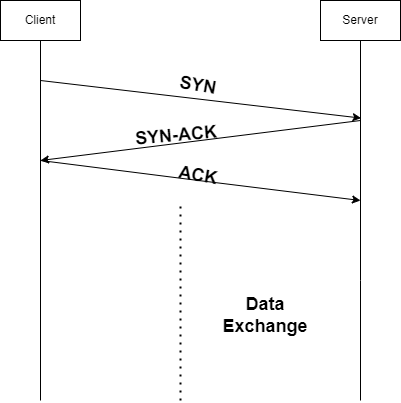
\includegraphics[width=0.45 \textwidth]{images/TCP_start.png}}
\hspace{1.0cm}
\subfloat{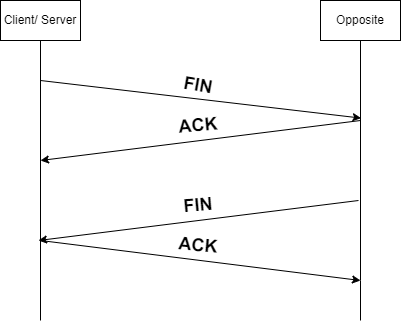
\includegraphics[width=0.45 \textwidth]{images/TCP_finish.png}}
\caption{Start (left) and End (right) of a TCP connection}
\label{fig:tcp}
\end{figure*}

If one side (the server or the client) wants to finish the connection \cite{Blog_ClosingTCPSession} and sends no more data, it sends a finsh packet (FIN) to the opposite. The opposite confirms that it received the FIN packet by sending an ACK packet. Now the opposite sends a FIN packet back to the side which sent the first FIN packet and this side confirms the receipt of this FIN packet with an ACK packet as well. After this closing process, which is illustrated in figure \ref{fig:tcp} on the right, the opposite can close the connection. Another possibility to close a TCP connection is simply by sending an RST package to the opposite side and then the connection is closed. \cite{Blog_ClosingTCPSession} stated that during this process, many things can go wrong, which he called \textit{abnormal terminations}. Those abnormal terminations could be either an aborted setup or a disconnection and they could occur due to the following reasons: There could be a lack of resources or a network interruption could occur, the session could crash due to a bug in the implementation, one side has already closed the connection and the other side continues to send data, or the server refuses to establish a connection with the client. 

\section{DNS over HTTPS} \label{doh}
DNS over HTTPS (DoH) is a protocol used for the traffic of DNS queries using the HTTPS protocol which was first introduced in 2018. There are two different approaches of DoH, the first one uses DNS in wire-format encapsulated in HTTPS \cite{RFC8484}, the other one uses DNS represented in JSON format \cite{RFC8427}. Both approaches are supported by the majority of all implementations, but the more commonly used approach is DNS in wire-format \cite{BoettingerEtAl_CostOfDoH}, therefore the main focus of this Bachelor Thesis will be laid on the DNS in wire format approach. There are several public DoH servers \cite{Blog_DNSProviders} available, inter alia \textit{Cloudflare}, \textit{Google}, \textit{Quad9}, and \textit{AdGuard}.

\subsection{Strengths} \label{doh_strengths}
\cite{Lu2019LageScaleMeasurement} conducted a large-scale measurement of DNS-over-Encryption, inter alia of DoH. They stated that that the mixture of DoH queries with other HTTPS traffic effectively resits traffic analysis that only targets DNS queries. This improves the protection of the content of DNS queries and with it the privacy of the traffic significantly, in other words it becomes difficult for an attacker to get an insight of the DNS queries. Another point is that DoH demands both encryption and authentication of servers. If a server is unable to provide these two security measures, the DoH query will fail and no data exchange will take place between the respective server and the client. Due to this fact, already the detection of DoH servers becomes very challenging. \cite{NSA_AdoptingEncryptedDNS} stated further that the authenticated and encrypted responses form the servers are immune from unauthorized modification by attackers.

\subsection{Vulnerabilities} \label{doh_vulnerabilities}
DoH entails the benefit that the DNS traffic between client and resolver is protected from unauthorized access but this fact also leads to issues. \cite{NSA_AdoptingEncryptedDNS} presented the following issues:  DoH conveys a false sense of security, DNS monitoring can be bypassed, the DNS upstream can be exploited, and there are concerns for internal network configurations and information. DoH has a lot of properties that promise being absolutely protected against cyber attacks. But in return there are possibilities for an attacker to gain information about the connection the client made to the server. This leads to a false sense of security. DNS monitoring has the function to filter and stop traffic from known malicious domains. Using DoH makes it impossible for these monitoring services to have a direct insight into the plaintext DNS traffic. If now external DoH servers are used, attackers get the possibility to get insight into the encyrpted DNS traffic. If an organization uses a device or an application that is configured to use an external DoH server, it ignores internal security measures and connects directly to that external resolver. This fact is a huge concern for internal network configurations and information because if now the client wants to connect to an internal domain, the device or the application sends the query first to the preferred and external resolver before at worst failing the internal resolver. Thus it becomes possible that internal network information is revealed to a third party. DoH takes place only on the "last mile" between the client system which statrts the DNS request and the DoH server which is addressed by the client. If the DoH server transmits the traffic to top-level root DNS servers of the internet, it could occur that the traffic from this point is not encrypted anymore. Thus, an attacker exploit the upsteam DNS traffic and can here have an insight on the plaintext DNS traffic and can try to redirect the traffic to a malicious server.

\subsection{Malware} \label{malware}
As seen in the previous Section, DoH is not fully secure. On this account, there have recently already been cyber attacks that abuse the security properties of DoH, in particular the fact that there is no possibility for insight into DoH traffic \cite{bumanglag2020ImpactOfDNS}. This Section creates an overview over the most common malware that abused the properties of DoH in the recent past, namely the Godlua Backdoor, PsiXBot, and Oilrig's APT34.

In April 2019, \cite{GodluaBackdoor} found a Lua-based Backdoor-file. Lua \cite{Lua} is a programming language which is according to \cite{shyhunt} a pretty popular and upcomming choice for web applications. A Lua-based Backdoor-file is a Lua Code Injection, which leaves a "backdoor" for an attacker to inject malicious queries into the affected web-application. Godlua Backdoor uses a redundant communication mechanism for C2 connections, where attackers use a combination of several ways to store a C2 address, and at the same time they use HTTPS and DoH to ensure the secure communications for their bots.

In early 2019, PsiXBot \cite{psixbot}, which uses Google's DoH service to get the domain name of Google's C2, was observed for the first time. With the knowledge of the domain name of the C2, PsiXBot can encrypt its DNS traffic and insert it masked into the normal HTTPS traffic and therefore circumvent the DNS firewalls.

Oilrig, also known as APT34 is an Iranian hacker group which became in 2020 the first of their kind to incorporate the DoH protocol into its attacks \cite{Oilrig}, using their until then newest tool, the \cite{DNSExfiltrator}. This tool is capable of transferring data between two points using the DoH protocol. Oilrig used this abilities to laterally shift data across an internal network to an exfiltration channel, where they could take data undetected from monitoring systems, using exactly the security property of DoH that does not allow to have an insight into the traffic.

\section{SecGrid} \label{secgrid}
SecGrid \cite{SecGrid} is a Machine Leaning empowered platform for the Analysis, Classification and Visualization of cyber-attacks. It is written in JavaScript (JS) and implements a set of miners, which are able to analyze network traffic files (i.e. PCAP-files \cite{pcap}) and gain an insight into possible attacking patterns and classify them. Furthermore, the suggested miners are extensible. It also uses the method \textit{Fast Flux} \cite{psixbot2}, which is a method to rapidly change the DNS entries by the usage of a Botnet to avoid being detected.

\begin{figure} [h]
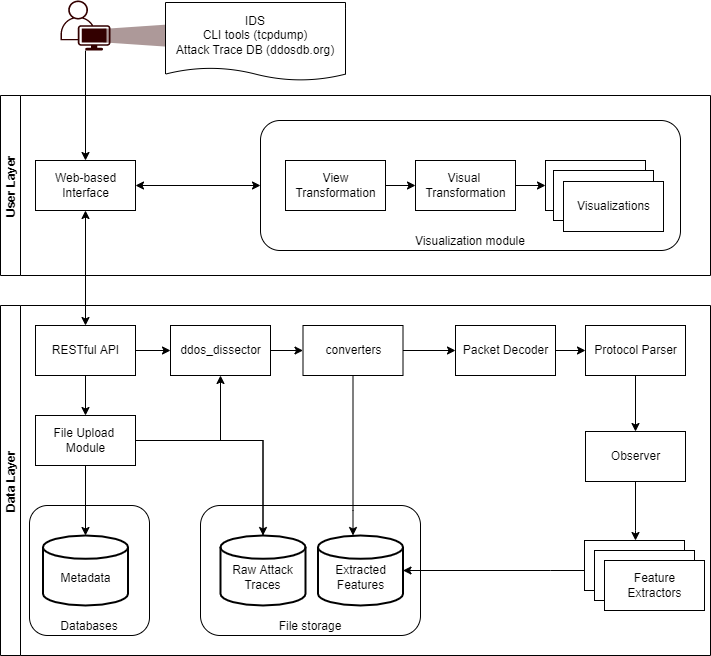
\includegraphics[scale=0.5]{current_architecture.png}
\centering
\caption{Current Architecture of SecGrid \cite{SecGrid}}
\label{fig:curr_arch}
\end{figure}

Figure \ref{fig:curr_arch} shows the current architecture of SecGrid. In the \textit{User Layer}, the user can choose already available data-sets or upload new ones to detect in the web-based interface. There the data is forwarded to the RESTFUl-API, which takes the part of the data manager in the \textit{Data Layer}. If a new data-set is uploaded, the data-manager forwards it to the data extraction pipeline where it gets analyzed and forwarded back to the \textit{User Layer}. In the \textit{User Layer}, the data get visualized in the \textit{Vizualization Module}, such that they deliver meaningful information to the user.

\section{PCAP-Files} \label{pcap}
Packet Capture (PCAP) \cite{pcap} files are used to capture live packet traffic data. The files can be generated with network analyzers like \textit{Wireshark} \cite{wireshark}. The packets in turn can be used to analyze the traffic which is done by the client. The features that are recorded in .pcap files are listed in Table \ref{tab:pcap_features}. Most of the features are self explanatory, like \textit{No.} (Number of the packet), \textit{Time}, \textit{Source}, \textit{Destination}, \textit{Protocol}, and \textit{Length}. The feature \textit{Info} contains the most important information about the packet, since here the user can see which type of message this packet is, e.g. in terms of the TPC protocol the .pcap file can capture if it was a SYN packet, or an ACK packet, etc. Figure \ref{fig:ex_pcap} shows the summary of the features of an example .pcap file parsed in \textit{Wireshark}. Other PCAP-parsers may extract slightly different features.

\begin{center}
\begin{longtable}{ |l|l| }
\hline
Feature & Explanation \\
\hline
\hline
No. & Number of the packet \\
\hline
Time & Time the packet was captured \\
\hline
Source & Source IP of the packet \\
\hline
Destination & Destination IP of the packet \\
\hline
Protocol & Protocol that was used for sending this packet\\
\hline
Length & Length of the packet (in bytes) \\
\hline
Info & Info about the packet \\
\hline
\end{longtable}
\captionof{table}{Features of a PCAP File in Wireshark}
\label{tab:pcap_features}
\end{center}

\begin{figure} [h]
\frame{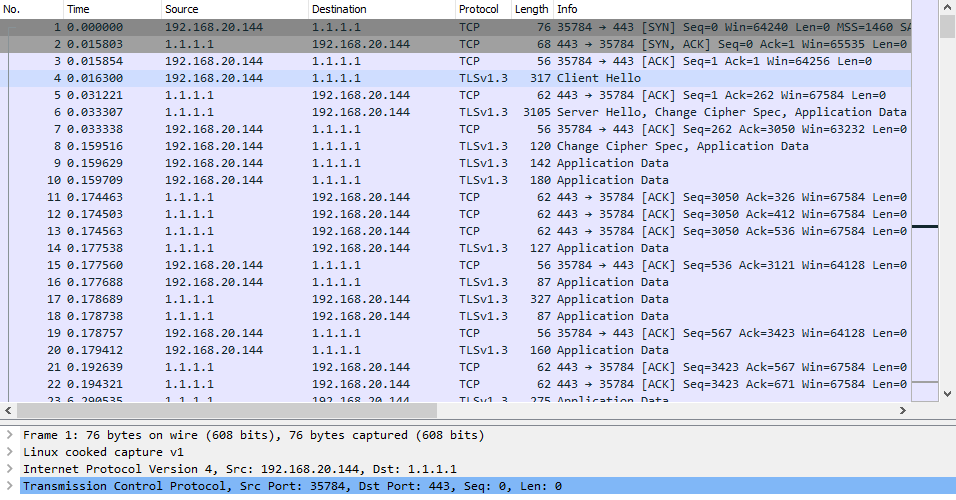
\includegraphics[scale=0.6]{images/pcap_file.PNG}}
\centering
\caption{Example PCAP File in Wireshark}
\label{fig:ex_pcap}
\end{figure}
